\documentclass[a4paper,11pt]{article}

\input ../include/preamble.tex

\usepackage{pgf-umlsd}
\usepgflibrary{arrows} % for pgf-umlsd
\usetikzlibrary{fit, positioning}

\begin{document}


\title{Pong - the first console game}

\author{Johan Montelius}
\date{Spring Term 2024}

\maketitle

\defaultpagestyle

\section*{Introduction}

This is an exercise in building an interactive game with two players
coordinated by one Elixir game engine. We will build the application
as a set of communicating processes where some processes are handling
the lower communication layers, one process is responsible for the
game logic and one to supervise and coordinate the actions. We will
use a web interface to handle the graphical display and forward input
from the players so there is some limited HTML and JS programming
involved.

The true reason why you want to do this exercise is of course that
the Pong game was a epic game, one of the first console games, that
changed the world for ever. 

\section*{The game of Pong}

The game of Pong is a very simple model of a game of tennis. The two
opponents can only move their paddle up and down along the base line
and the ball will bounce of the walls on the upper and lower side
walls. If a player fails to return the ball by having the paddle in
the right position she looses a point and the opponent gets to serve a
new ball.

A ball will bounce of the side walls in a perfect reflection but the
bounce from a paddle is slightly off depending on how far from the
center of the paddle that ball hits i.e. not the movement of the
paddle. This behavior will simulate spinning the ball and allows you
make a tougher return for the opponent to catch. 

\begin{figure}[t]
  \center 
  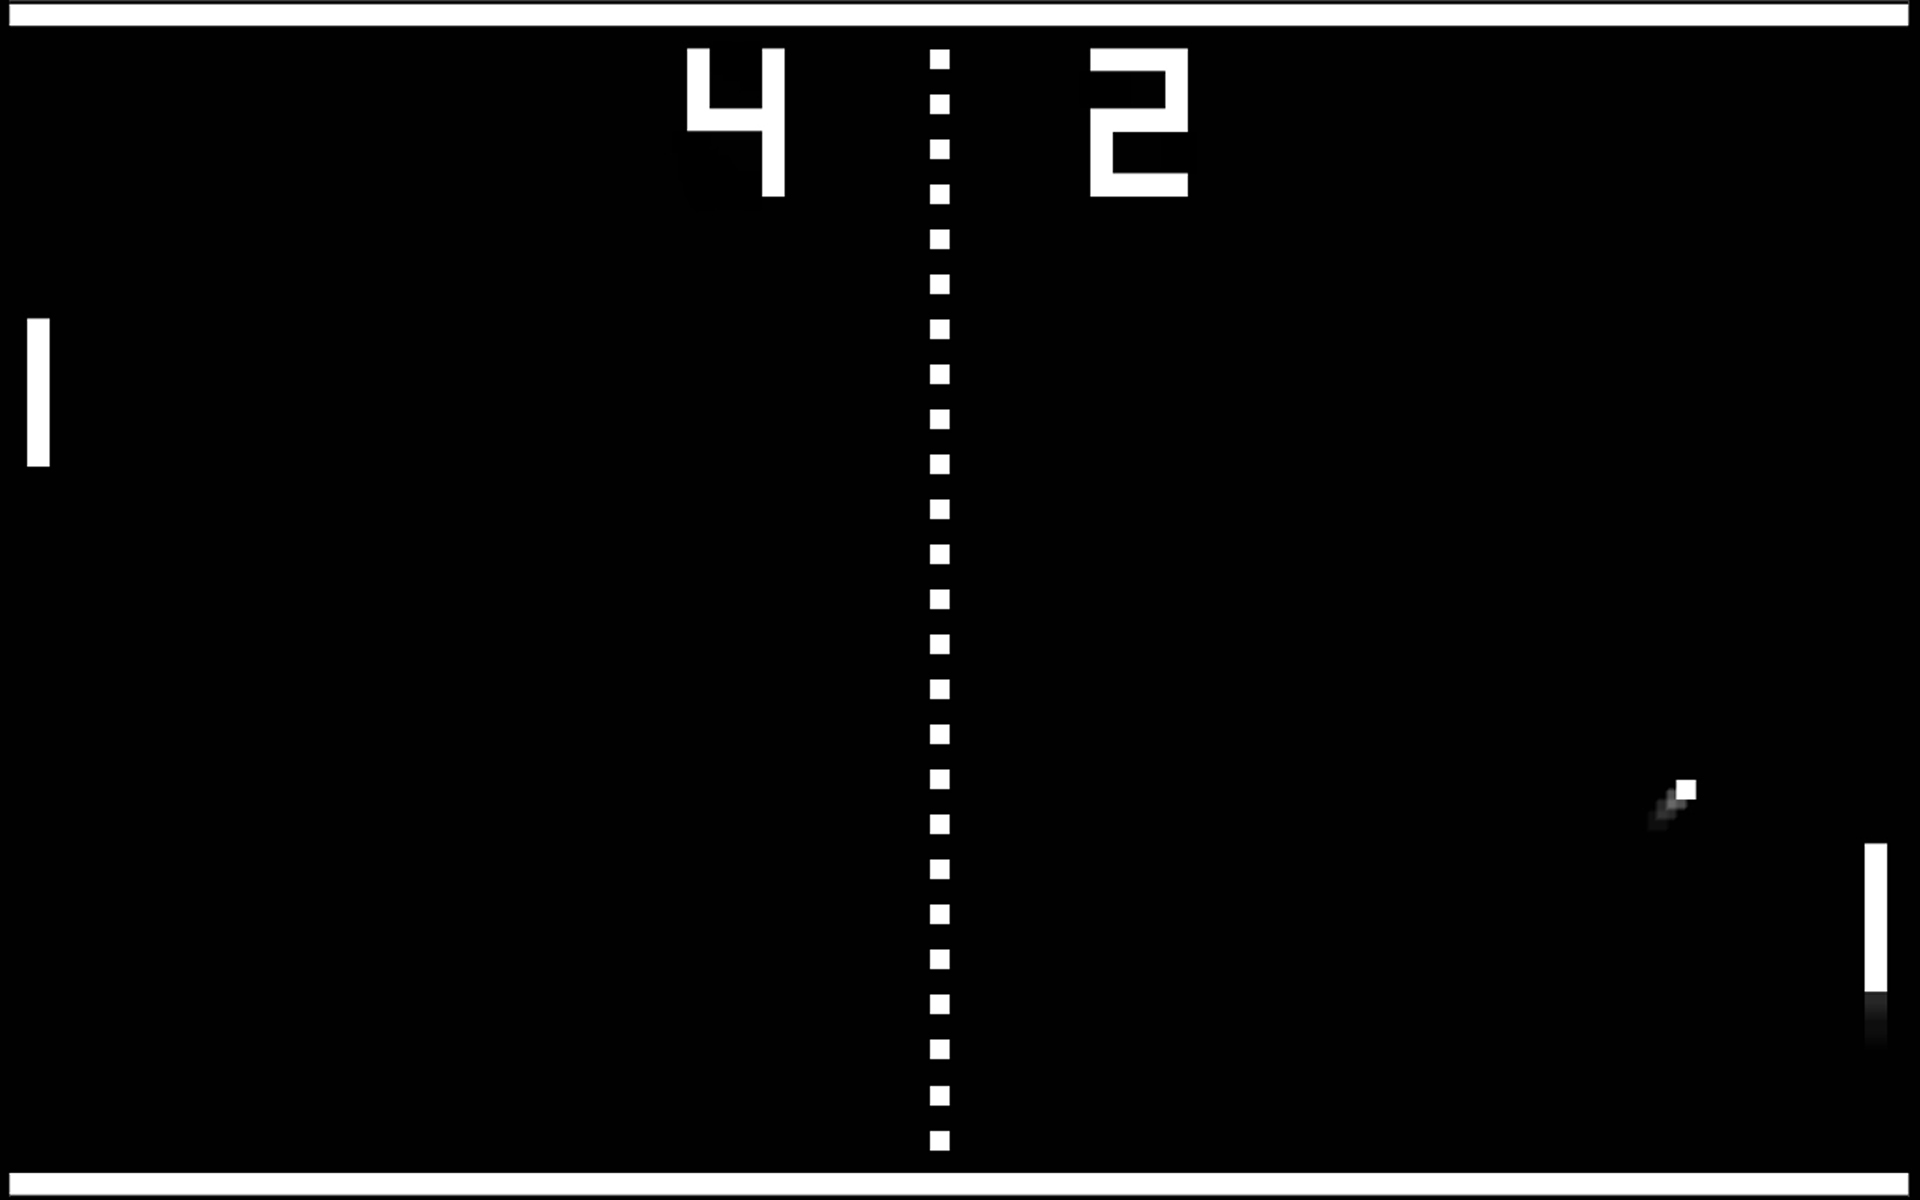
\includegraphics[scale=0.1]{pong.png}

  \caption{The game of Pong}
  \label{fig:pong}
\end{figure}

The classical Atari Game of Pong was played using a small console
attached to a TV. In our implementation we will of course use the
Internet and allow the two players to be anywhere as long as they have
a network connection. The look and feel should however be as in the
original version shown in Fig.~\ref{fig:pong}.

\section*{The architecture}
  
When we implement this game it is a lot easier to first divide the
system into processes that handle various aspects of the game. The
system will consist of: a client part, processes on the server side
that handles the communication with each player, a server process that
starts the game and keeps the game state and a module that describes
the rules of the game. The architecture is outlined in Fig.~\ref{fig:arch}. 

\subsection*{the client}

The client processes (browser 1 and 2 in Fig.~\ref{fig:arch}) will be
web browser that are responsible for displaying the game and forward
user interaction. The client behavior is implemented in JavaScript
and found in {\tt pong.js}. Since this is not a course in web design
we will keep it as simple as possible and I don't think we could do it
any simpler.

The communication between the clients and the server will be solved
using something called {\em web sockets}. This is a bidirectional
message protocol that is initiated through a HTTP request. On the
client side this will be handled by the JavaScript WebSocket library
but on the server side we will have to implement everything from
scratch (or use the version you will find in the git repo).

\subsection*{the server}

The heart of the system is the {\tt server} process. It is the process
that we first start and it is responsible for handling the game
state. To make the communication with the clients easier we add two
layers between the server and the clients. The low level details of
decoding and encoding websocket messages is handled by a {\tt handler}
process. It will deliver messages as byte sequences to a {\tt session}
process that will translate the byte sequences to more comprehensible
messages that are delivered to the server. The session process will
also encode messages from the server to byte sequences before sending
them to the handler process. 


\begin{figure}
  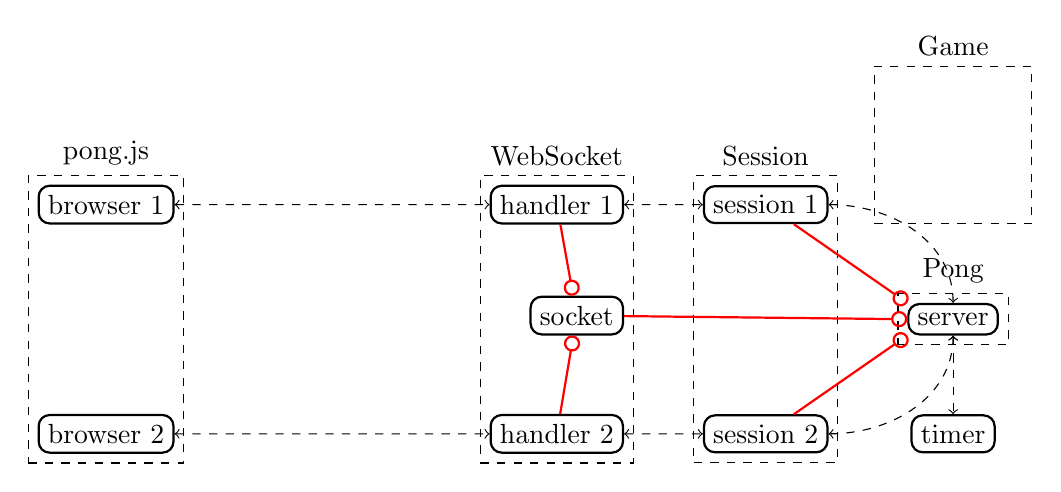
\begin{tikzpicture}[scale=0.6]
    \node[draw, thick, rounded corners] (server) at (0,0) {server};
    \node[draw, thick, rounded corners, above left = of server] (ses1) {session 1};
    \node[draw, thick, rounded corners, below left = of server] (ses2) {session 2};
    \node[draw, thick, rounded corners, below left = of ses1, above left = of ses2] (socket) {socket};
    \node[draw, thick, rounded corners, left = of ses1] (hdlr1) {handler 1};
    \node[draw, thick, rounded corners, left = of ses2] (hdlr2) {handler 2};
    \node[draw, thick, rounded corners, left = 4.0 cm of hdlr1] (brw1) {browser 1};
    \node[draw, thick, rounded corners, left = 4.0 cm of hdlr2] (brw2) {browser 2};
    \node[draw, thick, rounded corners, below = of server] (tmr) {timer};    

    \node[draw, dashed, fit = (server), label=Pong] {};
    \node[draw, dashed, fit = (ses1)(ses2), label=Session] {};
    \node[draw, dashed, fit = (socket)(hdlr1)(hdlr2), label=WebSocket] {};
    \node[draw, dashed, fit = (brw1)(brw2), label=pong.js] {};

    \node[draw, dashed, rectangle, label=Game, above = of server, minimum size=2cm] {};
    
    \draw[o-,thick, red] (server.west) -- (socket);
    \draw[o-,thick, red] (socket) -- (hdlr1);
    \draw[o-,thick, red] (socket) -- (hdlr2);
    \draw[o-,thick, red] (server.north west) -- (ses1);
    \draw[o-,thick, red] (server.south west) -- (ses2);            

    \draw[<->,dashed, black] (brw1) -- (hdlr1);
    \draw[<->,dashed, black] (brw2) -- (hdlr2);                    

    \draw[<->,dashed, black] (hdlr1) -- (ses1);    
    \draw[<->,dashed, black] (hdlr2) -- (ses2);

    \draw[<->,dashed, black] (ses1.east) to [out=0,in=90] (server.north);
    \draw[<->,dashed, black] (ses2.east) to [out=0,in=270] (server.south);
    \draw[<->,dashed, black] (server.south) to [out=270,in=90] (tmr.north);            
  \end{tikzpicture}
  \caption{The Pong architecture.}
  \label{fig:arch}
\end{figure}

The server process holds the state of the game and acts on either
client messages or clock ticks (which will move the ball forward) but
it does not know much about how the game actually work. The game logic
is all defined in a module called {\tt Game}. This is where we decide
what to do if a user wants to move up or down or what happens if the
ball has moved. The Game module will know everything about how large
the court is, how balls bounce etc, it's much easier to keep all of
the details in one module.

\subsection*{the websocket layer}

The server will start by creating two processes, one {\tt session}
process for each player. It will then create a {\tt socket} process
that is given the process identifiers of the two session
processes. The socket process will open a TCP listening socket on a
specified port and then spawn two processes that wait for incoming
connections.

To describe how the websocket protocol works in detail is a bit outside
the scope of this exercise so let's only go through it briefly. A
client will open a connection by opening a TCP connection and then
send special HTTP request. This request will specify that it wants to
communicate over the websocket protocol so the server responds and
then keeps the connection open.

The client and the server can then communicate by sending encoded
message. The body of a message is a byte sequence so it up to us to
come up with a encoding of our messages as a byte sequence.

In order to handle the incoming messages the handler process will
spawn a decoder process that will listen and decode messages coming
from the client. Some low level socket messages it can reply to itself
but when it has received a proper message it will send it to the
handler process.

The handler process will receive messages from the decoder process and
forward them to its session process. If the decoder process detects
that the socket is closed it will inform the handler who then will
relay this information to the session process and then terminate.

The reason why the handler process chooses to spawn a decoder process
is that if it would read from the socket itself, it would be suspended
waiting for messages on the socket. A message from the session process
could then be delayed and not delivered in time. There are other ways
to solve this but in this situation it is easier to spawn a new
process that suspends reading from the socket while the handler
process is ready to receive messages from either the decoder or the
session process.

\subsection*{the session layer}

In Fig.\ref{fig:seq} the initialization of the system is shown. The
server process is started first and it spawns two session processes
giving them unique names ({\tt :player1}, {\tt :player1}). The server
then spawns the {\tt websocket} process that opens the specified TCP
port. The process is also given the process identifiers of the two
session processes. The websocket process then spawns the two handler
processes that will, when they receive a connection, report back to
their session processes that they are open. 

Once the session process receives the messages from a handler process
it will report back to the server process that it is ready to start
the game. The server process will wait for both session processes to
report and can then serve the first ball. 

During the game the session process is responsible for encoding and
decoding messages between the pong server and the client browser.

The messages from the handler process to the session process are as follows:

\begin{itemize}
\item {\tt \{:ws, pid, :open\}}  : a connection was establishes
\item {\tt \{:ws, pid, :close\}} : the connection was closed by the client
\item {\tt \{:ws, pid, \{:msg,  <<?U, _::binary>>\}\}} : player pressed up arrow
\item {\tt \{:ws, pid, \{:msg,  <<?D, _::binary>>\}\}} : player pressed down arrow
\end{itemize}

The messages generated when the player presses either the up or down
arrow are decoded and delivered to the pong server as {\tt\{:pong1,
  :up\}} and {\tt\{:player1, :down\}}. The session process knows if it
is handling {\tt :player1} or {\tt :player2} and can thus generate the
right messages. Note that the client process can not decide by its own
that a paddle should be moved, it only passes the request to move to
the pong server. It is the server that decides in what order things
should move.

The pong server constantly send messages to the client, directing it to
move paddles, the ball or update the score. These messages needs to be
encoded as byte sequences. These are the messages from the pong server
and how they are encoded:

\begin{itemize}
\item {\tt \{:player1, :up\}}  : player 1 moved up -  {\tt <<?P,?U>>}
\item {\tt \{:player1, :down\}}  : player 1 moved down - {\tt <<?P,?D>>}
\item {\tt \{:player1, :score, score\}}  : player 1 new score - {\tt <<?P,?S, score>>}
\item {\tt \{:player2, ... \}} : same messages for player 2 -  {\tt <<?O, ... >>}        
\item {\tt \{:ball, x, y \}} : ball moved  - {\tt <<?B, x::16, y::16 >>}        
\item {\tt \{:ball, :hide\}} : hide ball - {\tt <<?B, 0::16, 0::16>>}        
\item {\tt \{:frw, msg\}}  : raw message to client - {\tt msg}
\end{itemize}

The raw message is used for debugging, a possibility for us to
communicate directly with the client.

\begin{figure}
\center
\begin{tikzpicture}[scale=1]

  \coordinate (n0) at (0,6);
  \coordinate (nn) at (0,-0.5);

  \coordinate (a0) at (3, 3);
  \coordinate (an) at (3,-0.5);

  \coordinate (b0) at (5,4);
  \coordinate (bn) at (5,-0.5);

  \coordinate (c0) at (7,5);
  \coordinate (cn) at (7,-0.5);

  \coordinate (s0) at (12,6);
  \coordinate (sn) at (12,-0.5);

  \draw[->] (n0) to []  (nn);
  \draw[->] (s0) to []  (sn);

  \node[anchor=south] at (n0) {browser 1/2};
  \node[anchor=south] at (s0) {pong server};

  \coordinate (s2) at ($(s0)+(0,-1)$);
  \draw[dashed] (s2) -- node[near start, above]{start(name, me)\ \ } (c0);
  \node[anchor=south] at (c0) {session 1/2};  
  \draw[->] (c0) to []  (cn);

  \coordinate (s3) at ($(s2)+(0,-1)$);
  \draw[dashed] (s3) -- node[near start, above]{start(8080,[ses1, ses2])\ \ } (b0);
  \node[anchor=south] at (b0) {websocket};  
  \draw[] (b0) to []  ($(b0)+(0,-2)$);

  \coordinate (b1) at ($(b0)+(0,-1)$);
  \draw[dashed] (b1) -- (a0);        
  \node[anchor=south] at (a0) {handler 1/2};  
  \draw[->] (a0) to []  (an);  

  \coordinate (n4) at ($(n0)+(0,-4)$);
  \coordinate (a1) at ($(a0)+(0,-1)$);
  \draw[dashed, <->, shorten <=0.2cm, shorten >=0.2cm] (n4) -- node[midway, above] {websocket} (a1);

  \coordinate (a2) at ($(a1)+(0,-1)$);
  \coordinate (c2) at ($(c0)+(0,-4)$);
  \draw[->, shorten <=0.2cm, shorten >=0.2cm] (a2) -- node[midway, above] {\{:ws, pid, :open\}} (c2);

  \coordinate (c3) at ($(c2)+(0,-1)$);
  \coordinate (s4) at ($(s3)+(0,-4)$);
  \draw[->, shorten <=0.2cm, shorten >=0.2cm] (c3) -- node[midway, above] {\{:ready, name\}} (s4);  
\end{tikzpicture}
\caption{A sequence diagram showing how the communication layer is started.}
\label{fig:seq}
\end{figure}

\subsection*{the pong server}

Once we have the session layer working we can concentrate on building
the game engine. The pong server needs to have a model of the game
state, know how to change it based on requests and broadcast the
changes to both players. The initial state of the game also needs to be
know by both clients so that the server only needs to inform the
clients of changes.

Since the rules of the game are quite extensive and needs to decide
what should happen each time the ball moves or a player wants to move
we implement this in a module of its own. The pong server will thus
know very little about what is going on and always consult the game
module before acting on a request. 

The state of the game is simply keeping track of where the players
have their paddles, where the ball is and what the score is. The
server also holds the process identifiers of the session processes to
be able to broadcast the state changes.


\begin{itemize}
\item Two players ({\tt player1} and {\tt player2}).
\item A ball.
\item The current score.
\item Two {\em session pids} to send messages to the players. 
\end{itemize}

The message that come from the session processes are request to move
the paddles. The game module is use to determine if the move is
possible and if so, an directive to move the paddle is broadcasted to
the session processes. Note that the server always broadcast the
changes to both clients, the clients thus receives the same messages
from the server.

\begin{minted}{elixir}
  def pong(player1, player2, ball, score, sessions) do
    receive  do

      {:player1, :down} ->
	case Game.down(player1) do
	  {:ok, player1} ->
	    broadcast(sessions, {:player1, :down})
	    pong(player1, player2, ball, score, sessions)
	  :no ->
	    pong(player1, player2, ball, score, sessions)
	end
      :
      :
    end
 end
\end{minted}


Moving the paddles in the simple problem to solve, it's a bit trickier
to handle the ball. In order for the ball to move the sever must
periodically calculate the new position of the ball and then update
the clients. This is solved using a call to {\tt :timer.send_after/3}
function. This function will schedule a message to a process after a
given time and we set this up to send a {\tt :tick} message after
$100 ms$. When the tick message is handled the ball is moved and a new
tick message is scheduled.


\begin{minted}{elixir}    
        :
      {:tick, tick} ->
	
	case Game.move_ball(player1, player2, ball) do
	  {:moved, pos,  ball} ->
	    :timer.send_after(tick, self(), {:tick, tick})
	    broadcast(sessions,  {:ball, pos})
	    pong(player1, player2,  ball, score, sessions)

          :
        end
      :
\end{minted}
    
The last message we need to handle is a {\tt \{:serve, :player1\}} (
or {\tt :player2}) message. This is also a message that the server
schedules to be sent to itself after a second or two. When it is
received a new ball is generated and the games starts. Every time a
player misses the ball a new serve message is scheduled.

\begin{minted}{elixir}    
        :
      {:serve, :player1} ->
	{pos, ball}  = Game.serve(player1)
	tick = @tick
	:timer.send_after(tick, self(), {:tick, tick})
	broadcast(sessions, {:ball, pos})	
	pong(player1, player2, ball, score, sessions)
      :
\end{minted}

The pong server also detects if any of the players stops
responding. The websocket handler will detect if a socket is closed
and will inform the session handler. The session handler will then tell
the pong server that is it terminating.

\begin{minted}{elixir}    
        :
      {:player1, :close} ->
	:io.format("pong: player 1 closed connection\n" )
	:ok
      :
\end{minted}

The pong server will thus when created:

\begin{itemize}
\item Start two session processes.
\item Start a websocket process and ask it to connect two handlers to the session processes.
\item Wait for both session handlers to report when they have a
  connection to a client browser.
\item Create two players and set the timer to delver a serve message.
\item Respond to messages from the session handlers and broadcast
  state updates.
\end{itemize}

Once a player quit, or we send a {\tt :stop} message, the pong server
terminates and closes the session handlers and the websocket process.


\subsection*{the game module}

The game module is responsible for the rules of the game, it does not
know that we play a game and is only there to answer questions what
should happen next. How the game state is represented is up to the
module and should stay inside the module.

The functions exported from the game module are the following:

\begin{itemize}
\item {\tt player1(name)} : return player one given a name. The name
  will later be used to indicate if the player scored a point. The
  player data structure will hold information about the position of
  the paddle and if the player is to the left or right.

\item {\tt player2(name)} : return player two given a name. Player two is 
  of course positioned at the other side of the board.

\item {\tt down(player)} : the player wish to move down, return either
  {\tt \{:ok, updated\}} if the player can move down or {\tt :no} if
  the player is already at the lower end of the board.

\item {\tt up(player)} : same thing but now the player wants to move up.

\item {\tt serve(player)} : the player serves the ball, return a tuple
{\tt \{position, ball\}} where the position is the x-y coordinates of
the ball. This requires that we have encoded in the player if it is
the left or right player.

\item {\tt move_ball(player1, player2, ball)} : this is the function
  that describes much of the game. The ball should move forward
  i.e. the ball needs encode both its direction and how far it should
  move. Many things can now happen depending on if the ball hits a
  wall, a paddle or simple scores a point. The state of the games,
  apart from the size of the board must be encoded in the data
  structures of the players and the ball. The returned value is
  either:

  \begin{itemize}
  \item {\tt \{:moved, pos, ball\}} : if the ball simply moved forward to a new position.
  \item {\tt \{:score, name\}} : if a player scored a point.
  \item {\tt \{:bounced, pos, ball\}} : the ball bounced against a
    paddle and we might want to increase the speed.
  \end{itemize}

\end{itemize}

Once we have all the pieces of the puzzle we can enjoy a game of pong. 


\end{document}
